\documentclass[a4paper,12pt]{article}

\usepackage[utf8]{inputenc}
\usepackage{graphicx}
\usepackage[dvipsnames]{xcolor}

%\usepackage[defaultmono]{droidmono}
\usepackage{wrapfig}
\usepackage{caption}
\usepackage{subcaption}

\usepackage{amsmath,amssymb,amsthm,textcomp}
\usepackage{ dsfont }
\usepackage{enumerate}
\usepackage{multicol}
\usepackage{tikz}
\usepackage{listings}
%\usepackage{pst-plot}
\usepackage{geometry}
\usepackage{sidecap}
\geometry{total={210mm,297mm},
left=25mm,right=25mm,%
bindingoffset=0mm, top=20mm,bottom=20mm}


\linespread{1.3}

\newcommand{\linia}{\rule{\linewidth}{0.5pt}}

%\savedata{\data}[{{0,0},{1,1},{2,11},{3,6},{4,6},{5,3},{6,2},{7,0},{8,0},{9,1},{10,1},{11,0},{12,1},{13,0},{14,0},{15,0},{16,1},{17,1}}]

%\renewcommand\lstlistingname{Code}

\definecolor{backcolour}{rgb}{0.95,0.95,0.95}

\lstset{%
    backgroundcolor=\color{backcolour},
    basicstyle=\ttfamily\small,
    breaklines=true,
    captionpos=t,
    numbers=left,
    numberstyle=\small,
    numbersep=5pt,
    frame=tb,
    commentstyle=\color{PineGreen},
    keywordstyle=\color{RoyalBlue}
}

% custom theorems if needed
% my own titles
\makeatletter
\renewcommand{\maketitle} {%
\begin{center}
\vspace{2ex}
{\huge \textsc{\@title}}
\vspace{1ex}
\\
\linia\\
\@author \hfill \@date
\vspace{4ex}
\end{center}
}
\makeatother
%%%

% custom footers and headers
\usepackage{fancyhdr}
\pagestyle{fancy}
\lhead{}
\chead{}
\rhead{}
\lfoot{HPSC \textbar \ Final Assignment}
\cfoot{}
\rfoot{15M54097 - Page \thepage}
\renewcommand{\headrulewidth}{0pt}
\renewcommand{\footrulewidth}{0pt}
%

% code listing settings
%%%----------%%%----------%%%----------%%%----------%%%

\newcommand*{\quoteTitle}[1]{{#1}\ignorespaces}%
\newenvironment{Quote}[1]{
    \medskip\par\noindent\quoteTitle{#1}
    \par\noindent
    \begin{quote}
    }{
    \end{quote}
    \par\noindent\ignorespacesafterend
}

\newtheorem{theorem}{Theorem}

\begin{document}
\bibliographystyle{acm}
\title{HPSC - Final Assignment}

\author{NGUYEN T. Hoang - SID: 15M54097}

\date{Spring 2016, W831 Mon-Thu. Period 1-2 \\ \hfill Due date: 2016/06/06}

\maketitle

\vspace{8em}
\section*{Problem}
\noindent
Solve the Laplace equation using multigrid.
$$\frac{\partial^2p}{\partial x^2} + \frac{\partial^2p}{\partial y^2} = 0,$$
in a $x=[0,2]$, $y=[0,1]$ domains with boundary conditions:
\begin{equation*}
    \begin{aligned}
        p=0 \ & at\ x=0,\\
        p=y \ & at\ x=2,\\
        \partial p / \partial y = 0 \ & at\ y=0,1.
    \end{aligned}
\end{equation*}

Modify the code in \texttt{demo.py} so that it runs with the sparse matrix from \texttt{step1.py}.

\vspace{10em}
\noindent
\emph{The source code and jupyter notebook for this assignment can be found at:} \\
\texttt{https://github.com/gear/HPSC/tree/master/hw}
File name: \texttt{assign2\_worksheet.ipynb}
\pagebreak
\section*{Answer}

\noindent
Using the given code in \texttt{step1.py}, I have the matrix $A$, vector $b$. This procedure is rewritten in \texttt{assign2\_worksheet.ipynb} as \texttt{laplace\_eq}.

\begin{lstlisting}[language=Python, caption={Solving Laplace equation using pyamg}, label={lst:border}]
     # Extracted from assign2\_worksheet.ipynb
     def amg_solver(A, b, cg=False, name='amg', tol=1e-10):
       mls = rootnode_solver(A)
       print mls
       # Solve Ax = b
       residuals = []
       if cg:
           x = mls.solve(b, tol=tol, accel='cg', residuals=residuals)
       else :
           x = mls.solve(b, tol=tol, accel=None, residuals=residuals)
       # Compute relative residuals
       residuals  = numpy.array(residuals)/residuals[0]  
       # Plot convergence history
       import pylab
       pylab.figure()
       pylab.title('Convergence History (%s)' % name)
       pylab.xlabel('Iteration')
       pylab.ylabel('Relative Residual')
       pylab.semilogy(residuals,  label='Residual',  linestyle='None', marker='.')
       pylab.legend()
       pylab.show()
\end{lstlisting}
\pagebreak
The result plots:
\begin{figure*}[h!]
  \centering
  \begin{subfigure}[b]{0.8\textwidth}
    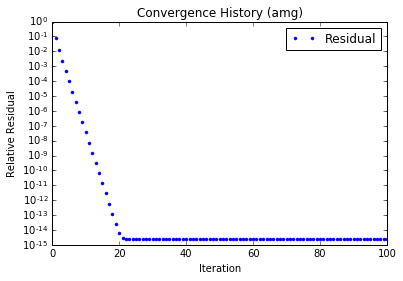
\includegraphics[width=\textwidth]{hpsc_final_nocg.png}
    \caption{Convergence of AMG without CG method.}
  \end{subfigure}
~
\begin{subfigure}[b]{0.8\textwidth}
    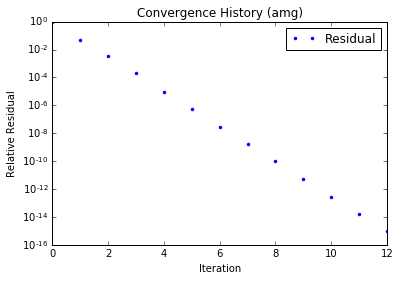
\includegraphics[width=\textwidth]{hpsc_final_cg.png}
    \caption{Convergence of AMG with CG method.}
  \end{subfigure}
  \caption{Convergence of AMG.}
\end{figure*}

\end{document}
